\section{Opera��es Suportadas}

Segue-se a descri��o de direc��es suportadas pelas opera��es, como ilustrado
na figura \ref{fig:shots}.

\subsection{Altera��o da Geometria}

\textbf{Extrus�o} --
direc��o definida pela compara��o com as normais da face origem.
Comprimento baseado no comprimento do tra�o.


\textbf{Bevel} --
a dimens�o do \textit{bevel} � dependente do comprimento do tra�o.


\textbf{Mover Face} --
suporta n�o s� as direc��es normais como tamb�m as co-lineares com as arestas fronteira da face.


\textbf{Mover Aresta} --
suporta as normais � aresta e as direc��es das faces vizinhas da mesma.


\textbf{Corte de Aresta} --
processa-se imediatamente, propagando o corte por arestas opostas at� terminar o \textit{loop} de face.

\subsection{Outras opera��es}

\textbf{Anular Opera��o} --
todas as opera��es desde a instancia��o do objecto podem ser revertidas.

\textbf{Salvaguarda e carregamento} --
o objecto pode ser guardado num formato simples em XML.
A exporta��o de conte�do a partir de pacotes de modela��o � poss�vel,
tendo sido implementado um \textit{plug-in} para Blender.

\begin{figure}[!ht]
	\centering
	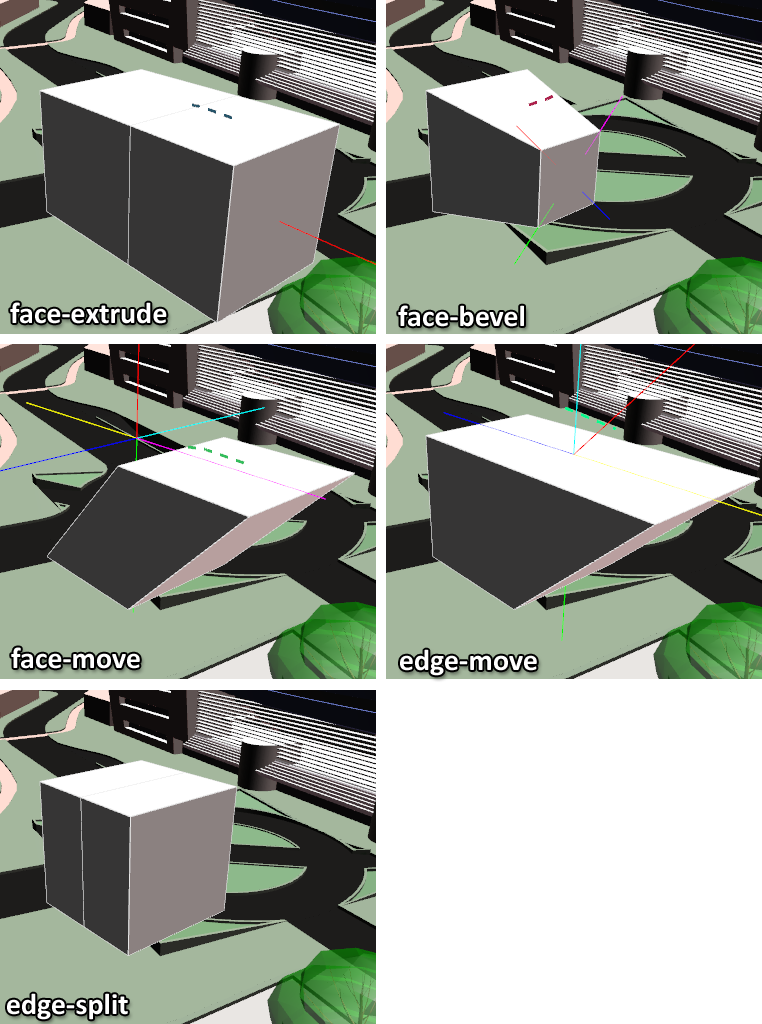
\includegraphics[width=0.8\linewidth]{shots2.png}
	\vspace{-3mm}
	\caption{opera��es no ImmiView}
	\label{fig:shots}
	\vspace{-3mm}
\end{figure}